%%%% NeurReps Extended Abstract track — OFFICIAL template (jmlr.cls from
%%%% the NeurReps style zip; see VENUE_REQUIREMENTS.md). This build is the
%%%% ANONYMIZED review version: per the template instructions no author
%%%% block appears at all during review; camera-ready uncomments it.
%%%%
%%%% TITLE: PENDING-USER (PI decision). Candidate (A) typeset; candidate
%%%% (B) in brief.md.
%%%% AUTHOR BLOCK: PENDING-USER — commented camera-ready placeholder below.
%%%%
%%%% The CFP asks for a single .tex file at submission: `make bundle`
%%%% writes the flattened bundle/neurreps-ea-submission.tex from this
%%%% modular source.
\documentclass[mlabstract,onecolumn]{jmlr}

%%%%%%%%%%%%%%%%%%%%%%%%
% Watermark (review builds only; remove for camera-ready)
% (the sample zip writes hpos=300px,vpos=70px; px is a pdfTeX-only unit and
% this build engine runs XeTeX, so the equivalent bp values are used --
% 1px = 1bp at pdfTeX's default \pdfpxdimen)
\usepackage[hpos=300bp,vpos=70bp]{draftwatermark}
\SetWatermarkText{\test}
\SetWatermarkScale{1}
\SetWatermarkAngle{0}
%%%%%%%%%%%%%%%%%%%%%%%%

% The class auto-loads: amsmath, amssymb, natbib, graphicx, url, algorithm2e.
\usepackage{booktabs}

\graphicspath{{figures/}}

\theorembodyfont{\itshape}
\theoremheaderfont{\bfseries}
\newtheorem{fact}{Fact}

\newcommand{\R}{\mathbb{R}}
\newcommand{\rank}{\operatorname{rank}}
\newcommand{\dmin}{d_{\min}}
\newcommand{\dstate}{d_{\mathrm{state}}}
\newcommand{\recninety}{\mathrm{rec}@0.9}

%%%% DON'T CHANGE %%%%%%%%%
\jmlrvolume{}
\firstpageno{1}
\editors{Under Review for the NeurReps Workshop}
\jmlryear{2026}
\jmlrworkshop{Symmetry and Geometry in Neural Representations}
%%%%%%%%%%%%%%%%%%%%%%%%%%%

\title[A Causal Rank Law for Matrix Memories]{The Rank the Task Demands:
A Causal Rank Law for Matrix Memories Trained on Group Composition}

% CAMERA-READY ONLY (PENDING-USER): uncomment and fill after acceptance.
% \author{\Name{Author Name(s) TBD} \Email{email@TBD}\\
% \addr Affiliation TBD}

\begin{document}

\maketitle

\begin{abstract}
Matrix-valued memories make rank the natural budget of a learned
representation: the number of independent directions a state spans bounds
what it can bind, compose, and track. We report causal evidence, from two
synthetic testbeds trained under a hard single-state bottleneck with an
exact-continuous-recovery readout, that gradient descent recruits precisely
the rank the task's algebra demands. On $K$-pair associative binding, where
exact recovery provably requires state rank at least $K$, trained states
develop effective rank tracking $K$ (8.20 at $K{=}8$, 15.08 at $K{=}16$ for
$d{=}16$), and train-time rank caps confirm the bound causally: at $d{=}8$,
$K{=}4$, rank 3 yields zero exact recovery while rank 4 yields 0.94. On
group-composition state tracking over five groups spanning the
solvable/non-solvable divide, the recruited rank equals the group's minimal
faithful real representation dimension $\dmin$ (Spearman $\rho = 0.9747$,
the design's tie-capped maximum), the dimension-matched solvable/non-solvable
pair $S_4$/$A_5$ is statistically equivalent under a pre-registered
equivalence test, and a force-rank razor lands a step function at $\dmin$ in
all five groups: one rank below, exact recovery is 0.000 everywhere,
including every seed of a four-seed extension, while at $\dmin$ recovery
returns to unconstrained-anchor levels. Representation theory, not
computational complexity class, sets what gradient descent buys.
\end{abstract}

\begin{keywords}
effective rank, fast weights, group representations, state tracking
\end{keywords}

\section{Introduction}
\label{sec:intro}

A matrix-valued memory represents by spanning: whatever a $d \times d$
state binds or tracks, it holds in the geometry of its column space, and
rank is the budget it spends. Prior work treats this budget
descriptively \citep{nazari2026rank, sun2026staterank} or through
hand-built constructions \citep{nichani2025factual}; neither answers
what a geometric account of learned representations needs answered:
when a task's algebra fixes a minimal representational dimension, does
gradient descent recruit exactly that dimension, and is it causally
load-bearing?

We answer both halves affirmatively under one discipline: a hard
single-state bottleneck (the decoder reads only one matrix $Z$, verified
by a gradient blank-out test) and exact-continuous-recovery scoring
(cosine against the true continuous target, never argmax over a codebook,
which would let a rank-1 state recover on the order of $d$ associations
\citep{nichani2025factual}). Section~\ref{sec:setup} includes the
provable $K$-pair-binding foundation. The headline is
group-composition state tracking, where representation theory
supplies the ground truth: across five finite groups spanning the
solvable/non-solvable divide, the minimal faithful real representation
dimension $\dmin$ predicts the recruited rank almost perfectly, a
matched-dimension solvable/non-solvable pair lands statistically
equivalent (Section~\ref{sec:observed}), and a pre-registered force-rank
razor finds recovery exactly 0.000 one rank below $\dmin$ in every group,
returning at $\dmin$ (Section~\ref{sec:razor}): $\dmin{-}1$ is fatal,
$\dmin$ suffices. An earlier razor sweep nulled through an instrument
defect, an ambient identity block taxing every rank-capped arm; the
raw-artifact diagnosis, the registered inconclusive verdict, and the
repaired wave that landed the pre-registered prediction are part of the
result (Appendix~\ref{app:damb}).

\section{Tasks, Models, and the Rank Instrument}
\label{sec:setup}

\textbf{Tasks.} In the binding task, each episode presents $K$
key--value pairs, the encoder writes one state $Z \in \R^{d \times d}$,
prediction is the literal unbind $Z k_j$, and $\recninety$ is the
fraction of queries with cosine to the true value above 0.9. The group
task is the word problem of a finite group $G$: a word
$w = g_{i_1} \cdots g_{i_L}$, drawn as a random walk on $G$'s Cayley
graph ($L \sim \mathrm{U}\{1,\dots,8\}$), must map to
$\rho_G(g_{i_1} \cdots g_{i_L})$ under a pinned orthogonal reference
representation of dimension $\dmin(G)$, the minimal faithful real
representation dimension. The groups are $S_3, S_4, A_5, S_5, A_6$ with
$\dmin = 2, 3, 3, 4, 5$ (Appendix~\ref{app:groups}); the first two are
solvable, the rest are not, and non-solvable word problems are
$\mathrm{NC}^1$-complete \citep{barrington1989}. $\dmin$ is a different,
representation-theoretic axis; $S_4$/$A_5$, matched at $\dmin = 3$ with
opposite solvability, are the designed dissociation pair.

\textbf{Model.} A Transformer encoder with $\dstate$ learned row-reader
queries maps each word to a single state
$Z(w) \in \R^{\dstate \times \dstate}$, $\dstate = \dmin + 2$, leaving
spare dimensions so over-recruitment is expressible. The target embeds
the reference block-diagonally ($\rho_G(\cdot) \oplus I_2$ in the first
sweep, $\rho_G(\cdot) \oplus 0$ in the repaired wave); the loss is cosine
distance, the readout is fixed with no learned weights that could launder
rank, and the decoder reads only $Z$ (blank-out verified). Per-group
step budgets (8k--40k) were pinned by pre-registered convergence bars.

\textbf{Instrument.} The learned state is defined only up to scale and an
orthogonal change of basis (a Schur intertwiner):
$Z(w) \approx c\,Q\,[\rho_G(w) \oplus \cdot\,]\,Q^{\top}$. We estimate the
model's own dominant $\dmin$-subspace $U$ from the SVD of the
\emph{centered} covariance of $Z(w)$ over held-out words, measure
\textbf{restricted effective rank} (entropy effective rank of
$U^{\top} Z(w) U$), and score \textbf{degauged recovery}: cosine after
fitting $(c, Q)$ on a fitting split, evaluated on a disjoint split,
reported as $\recninety$. Centering is load-bearing
(Appendix~\ref{app:m1}); rank is invariant under the fitted gauge, so a
rank-deficient state cannot be degauged into a full-rank one. For force-rank cells the decisional readout was pinned, before
the razor wave ran, to the conservative full-$Q$ Procrustes variant
(\emph{crosscheck} $\recninety$).


\textbf{The provable foundation (binding).}
\begin{fact}
\label{fact:bound}
If $Z k_j = v_j$ exactly for $K$ bindings with linearly independent keys
and values, then $Z K_{\mathrm{mat}} = V_{\mathrm{mat}}$, so
$K = \rank(V_{\mathrm{mat}}) \leq \rank(Z)$.
\end{fact}

The bound is classical \citep{kohonen1972correlation,
anderson1972simple} and holds only under exact continuous recovery.
Gradient descent recruits the rank: at $d = 16$ the trained state's
effective rank reaches 8.20 at $K = 8$ and 15.08 at $K = 16$,
% <!-- evidence: N6 -->
and the recruited rank is causally necessary: a spectral rank cap at
$d = 8$, $K = 4$ leaves exact recovery at or below 0.0004 for every cap
$k \leq 3$ and restores it to 0.940 at $k = 4$,
% <!-- evidence: N6 -->
a step exactly at the provable bound; the same operator composes
exactly ($Z^h$, held-out depths to 21) in four of five seeds.
% <!-- evidence: N9 -->

\section{The Rank Law on Group Composition, Observed}
\label{sec:observed}

Figure~\ref{fig:tracking} (left) gives the observational leg: per-group mean
restricted effective rank lands within 4--8\% of $\dmin$ at every group,
and all 19 seeds sit inside the pre-registered $[0.7, 1.3] \cdot \dmin$
band (means and per-seed values in Appendix~\ref{app:m1}).
% <!-- evidence: N4 -->

Spearman correlation between recruited rank and $\dmin$ is
$\rho = 0.9747$,
% <!-- evidence: N4 -->
the maximum this design can express, since the $S_4$/$A_5$ tie caps
$\rho$ below 1; under the exact permutation null,
$P(\rho \geq 0.8) = 8/120 \approx 6.7\%$,
% <!-- evidence: N4 -->
so by pre-registration this leg is corroborating rather than independently
decisive (a disclosed length-robustness split is in
Appendix~\ref{app:m1}).

\textbf{Dimension, not solvability.} If recruited rank were set by
computational class, the marquee pair should separate; if by
representation dimension, coincide. A pre-registered Welch two-one-sided
equivalence test on restricted effective rank (margin $\pm 0.5$
rank-units, half the $\dmin$ ladder spacing; $n = 5$ per group; simulated
power 100\% to reject at a 1.0 rank-unit gap) observes a difference of
$+0.019$ rank-units (se 0.037, df 7.8), with both one-sided tests passing
at roughly seven times the critical value ($t = 13.06$ and $14.12$
against $t_{\mathrm{crit}} = 1.865$): equivalence is declared decisively.
% <!-- evidence: N5 -->
The pair lands together on dimension, where the rank law puts it.

\section{The Causal Razor}
\label{sec:razor}

The decisive test intervenes on rank: the encoder's output is
spectrally truncated to rank $k \in \{\dmin{-}1, \dmin, \dmin{+}1\}$
throughout training, against the zero-padded target
$\rho_G(\cdot) \oplus 0$ of rank exactly $\dmin$, alongside an
unconstrained anchor from the same family. Pre-registered reading: if
$\dmin$ is load-bearing, $k = \dmin{-}1$ must fail and $k \geq \dmin$
must recover past $0.9\times$ the anchor's crosscheck $\recninety$; a
single below-$\dmin$ cell recovering falsifies necessity.

\begin{figure}[t]
\centering
\begin{minipage}[c]{0.44\textwidth}
\centering
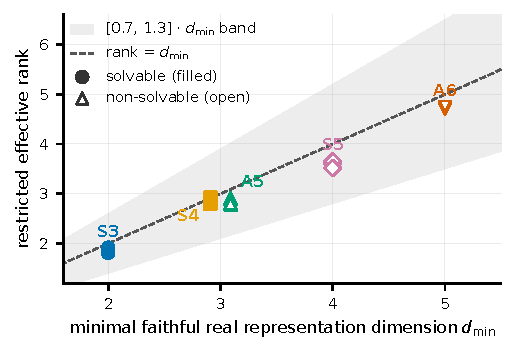
\includegraphics[width=\textwidth]{fig2_rank_tracking.pdf}
\end{minipage}\hfill
\begin{minipage}[c]{0.53\textwidth}
\centering
\small
\begin{tabular}{lccccc}
\toprule
$G$ & anchor & $k{=}\dmin{-}1$ & $k{=}\dmin$ & $k{=}\dmin{+}1$ & bar \\
\midrule
$S_3$ & 0.550 & 0.000 & 0.450$^{\ast}$ & 0.550 & 0.495 \\
$S_4$ & 0.650 & 0.000 & \textbf{0.800} & 0.950 & 0.585 \\
$A_5$ & 0.700 & 0.000 & \textbf{0.700} & 0.750 & 0.630 \\
$S_5$ & 0.500 & 0.000 & \textbf{0.600} & 0.550 & 0.450 \\
$A_6$ & 0.650 & 0.000 & \textbf{0.650} & 0.700 & 0.585 \\
\bottomrule
\end{tabular}
\end{minipage}
\caption{Left: recruited rank follows representation dimension, not
solvability. Each point is one seed's restricted effective rank vs.\ its
group's $\dmin$ (filled: solvable; open: non-solvable) with the
pre-registered $[0.7, 1.3] \cdot \dmin$ band and the identity line; all
19 seeds are in band, and $S_4$/$A_5$ coincide at $\dmin = 3$.
% <!-- evidence: N4 -->
Right: the causal razor on the repaired rank-$\dmin$ target (crosscheck
$\recninety$ by force-rank $k$, one seed per cell, unconstrained anchor,
pre-registered $0.9\times$anchor bar): exactly 0.000 one rank below
$\dmin$ everywhere, anchor-class at $\dmin$ (bold: clears the bar).
$^{\ast}$extended to four seeds under the pre-stated $\pm 0.05$ trigger:
seed-mean 0.5625 clears the fixed 0.495 bar.}
% <!-- evidence: N1 -->
\label{fig:tracking}
\end{figure}

\begin{figure}[t]
\centering

\includegraphics[width=\textwidth]{fig1_razor_step.pdf}
\caption{Exact recovery is a step function at $\dmin$: per group,
crosscheck $\recninety$ on held-out words at force-rank
$k \in \{\dmin{-}1, \dmin, \dmin{+}1\}$ (one seed per cell), vs.\ the
unconstrained anchor (dashed) and the $0.9\times$anchor bar (dotted).
$S_3$ overlays its four seeds (thin lines; bold mean); its
below-$\dmin$ zero is unanimous.}
% <!-- evidence: N1 -->
\label{fig:razor}
\end{figure}

Figure~\ref{fig:tracking} (right) and Figure~\ref{fig:razor} show the result on the
pre-pinned crosscheck readout. Necessity is exact and noiseless:
$k = \dmin{-}1$ yields $\recninety = 0.000$ in all five groups,
% <!-- evidence: N1 -->
and in all four independent seeds of the $S_3$ extension,
% <!-- evidence: N2 -->
while the same cells' recovery cosines (0.61--0.84) show the zero is a
threshold phenomenon, not a training collapse. Sufficiency holds at
$\dmin$: $S_4$, $A_5$, $S_5$, $A_6$ clear their bars outright,
% <!-- evidence: N1 -->
and $S_3$, whose decisive cell landed inside the pre-stated $\pm 0.05$
marginality trigger, was extended to four seeds under the trigger's
pre-registered routing: seed-mean 0.5625 against the fixed 0.495 bar
(the literal fixed before the extension ran, avoiding a self-referential
bar) confirms the fifth group.
% <!-- evidence: N3 -->
Both marquee groups confirm; the pre-registered causal criterion is met.

An earlier 58-cell sweep of this grid nulled through an instrument
defect: its eye-padded target ($\rho_G(\cdot) \oplus I_2$, rank $\dstate$)
taxed every capped arm, whose 39 cells sat at their rank-$k$ optimum
$\sqrt{k/\dstate}$ (mean deviation 0.028);
% <!-- evidence: N7 -->
that verdict was registered as inconclusive with the tax as mechanism,
and the zero-padded wave above is the registered fix
(Appendix~\ref{app:damb}).
% <!-- evidence: N8 -->

\section{Related Work and Limitations}
\label{sec:related}

\citet{nazari2026rank} and \citet{sun2026staterank} measure
effective-rank dynamics in pretrained linear-attention models,
observationally, with no task algebra fixing a required dimension;
\citet{mishra2026m2rnn} train matrix-state RNNs on $S_3$ composition but
measure no state rank and run no rank intervention.
\citet{grazzi2025negative}, \citet{siems2025deltaproduct}, and
\citet{merrill2024illusion} characterize which word problems recurrent
architectures can express, the solvability axis; the marquee equivalence
shows the \emph{learned geometry} sorts by representation dimension, not
that axis. A negative result on bolt-on matrix latents
\citep{larson2026gradient}, where a flatten-then-project readout makes
rank invisible to the gradient, is this result's negative counterpart.


\textbf{Limitations.} All results are on sub-1M-parameter synthetic
testbeds; nothing here is a claim about pretrained language models.
Over-recruitment beyond two spare dimensions is not expressible in this
state window; razor cells are single-seed except $S_3$ (four seeds;
necessity zeros exact wherever seeds exist); two groups at the shortest
pinned budget show soft convergence (disclosed; the razor reading is
anchor-relative and unaffected).

\appendix

\section{The Five Groups and Reference Representations}
\label{app:groups}

\begin{table}[h]
\centering
\small
\begin{tabular}{lcccl}
\toprule
$G$ & $|G|$ & $\dmin$ & solvable & realization of $\rho_G$ \\
\midrule
$S_3$ & 6   & 2 & yes & standard (dihedral) \\
$S_4$ & 24  & 3 & yes & cube rotations \\
$A_5$ & 60  & 3 & no  & icosahedral rotations \\
$S_5$ & 120 & 4 & no  & standard (zero-sum) \\
$A_6$ & 360 & 5 & no  & standard (zero-sum) \\
\bottomrule
\end{tabular}
\caption{The five task groups. $\dmin$ is the minimal faithful real
representation dimension; each reference representation is orthogonal by
construction and verified faithful (injective on $G$) at build time.
$S_4$/$A_5$ form the marquee pair: matched $\dmin$, opposite solvability.}
\label{tab:groups}
\end{table}

\section{Per-Seed Observational Rank}
\label{app:m1}

\begin{table}[h]
\centering
\small
\begin{tabular}{lccccc}
\toprule
$G$ & $\dmin$ & $n$ & restricted eff.\ rank & band & in band \\
\midrule
$S_3$ & 2 & 3 & $1.877 \pm 0.060$ & $[1.4, 2.6]$ & 3/3 \\
$S_4$ & 3 & 5 & $2.852 \pm 0.054$ & $[2.1, 3.9]$ & 5/5 \\
$A_5$ & 3 & 5 & $2.832 \pm 0.062$ & $[2.1, 3.9]$ & 5/5 \\
$S_5$ & 4 & 3 & $3.591 \pm 0.069$ & $[2.8, 5.2]$ & 3/3 \\
$A_6$ & 5 & 3 & $4.736 \pm 0.023$ & $[3.5, 6.5]$ & 3/3 \\
\bottomrule
\end{tabular}
\caption{Restricted effective rank of the unconstrained trained state
(mean $\pm$ sd over seeds) against each group's $\dmin$, with the
pre-registered $[0.7, 1.3] \cdot \dmin$ band. Every seed of every group is
in band; Spearman $\rho = 0.9747$ is the tie-capped maximum; the
dimension-matched pair $S_4$/$A_5$ differs by 0.019 rank-units.}
% <!-- evidence: N4 -->
\label{tab:m1}
\end{table}

The instrument's centering step is load-bearing: an uncentered lens
scores a flawless synthetic model 0.705 where the centered production
lens scores 0.9996 on identical data.
% <!-- evidence: N11 -->
The disclosed length-robustness split referenced in
Section~\ref{sec:observed} scores only words of length $L \geq 2$ (the
$L = 1$ read is attention-degenerate and was demoted with a mechanism
note in the run records): it moves per-group mean recovery cosine by at
most 0.013 (per-seed at most 0.041), with no group-selective divergence.
% <!-- evidence: N10 -->

\section{The Ambient-Identity Tax in Detail}
\label{app:damb}

The first sweep's force-rank target was the eye-padded
$\rho_G(\cdot) \oplus I_2$, whose rank is $\dstate = \dmin + 2$ for every
group. Because the identity block is constant across words, it is the
cheapest reliable loss reduction available, and a rank-capped arm buys it
before the group representation; the residual budget for $\rho_G$ is
$k - 2$, below $\dmin$ at every grid point, so no capped cell in the
original sweep ever tested the law's confirm direction. Three raw-artifact
signatures established this: (i) force-rank cells' direct cosine matched
the rank-$k$ optimum $\sqrt{k/\dstate}$ with mean absolute deviation 0.028
across all 39 cells (maximum 0.166; the two $S_5$ below-$\dmin$ cells are
the only outliers, an additional disclosed optimization shortfall), so the
arms trained to their rank-constrained ceiling rather than under-training;
% <!-- evidence: N7 -->
(ii) centered restricted rank of capped arms landed near $k - 2$, the
residual budget; (iii) in the repaired wave, an eye-padded corroboration
arm reproduces the failure on demand at raw $k = \dmin{+}1$ (effective
budget $\dmin{-}1$) while the tax-paid point recovers.
% <!-- evidence: N1 -->
The repaired wave's 30 cells were configuration-verified one-by-one
against a manifest re-derived independently from the design record (steps,
padding mode, and force-rank value per cell; zero skipped steps).
% <!-- evidence: N8 -->


\bibliography{refs}

\end{document}
